%!TEX output_directory = aux_dir
\documentclass[../SommerstjernerA4.tex]{subfiles}

\begin{document}
\section{Sommertriangelet}
Sommertriangelet er en asterisme\footnote{Et mønster av stjerner, enten i ett stjernebilde, eller over flere.} som består av stjernene Vega, Deneb og Altair i henholdsvis stjernebildene Lyren, Svanen og Ørnen. 

De tre stjernene i sommertriangelet er de første som blir synlige på stjernehimmelen om sommeren, og Vega er faktisk den femte mest lyssterke stjernen på himmelen. (Stjernen Arkturus som dere sikkert kjenner fra vårtriangelet er faktisk litt lysere, men er ganske nær solen om sommeren)

Triangelet er lett å finne på grunn av de lyse stjernene og på grunn av den sterke stjernen i nærheten av Altair, Tarazed ($\gamma$ Aquila).
\begin{figure}[bh]
\centering
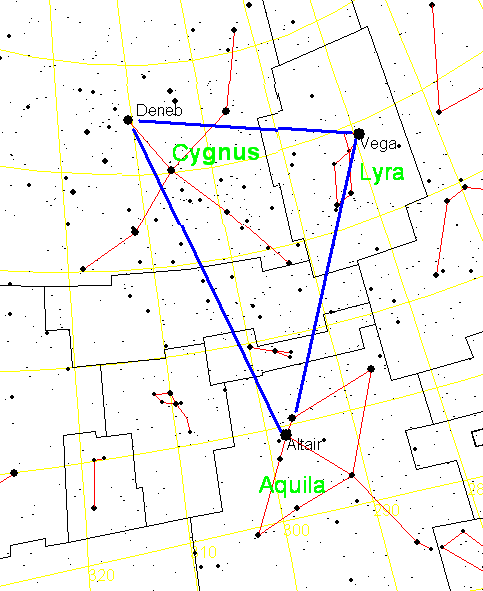
\includegraphics[width=0.5\textwidth]{Summer_triangle_map}
\caption{Kart over de tre stjernene i sommertriangelet. (Hentet fra Wikimedia Commons)}
\end{figure}

\subsection{Vega og Lyren}
Stjernen Vega ($\alpha$ Lyrae) er den sterkeste stjernen i stjernebildet Lyren (en håndholdt harpe). Vega er en av de sterkeste stjernene på himmelen (Nr. 2 på den nordlige halvkule), og er relativt nær jorden, bare 25 lysår.

Nordpolen på himmelen beveger seg i en sirkel på grunn av Jordens presesjon (det samme fenomenet som gjør at snurrebasser og fidget spinners\texttrademark{} ``peker'' rundt i en sirkel.) For 14000 år siden var Vega nordstjerne, og den kommer igjen til å være nordstjerne om ca. 12000 år.

Vega er også en ganske ung stjerne, som du kan se av den blå fargen. Den er omtrent ti ganger yngre enn solen. Den er også dobbelt så stor som solen.

Vega roterer veldig raskt og buler ut rundt ekvator. I motsetning til Jorden er det polene som er varmere enn ekvator, og det er den varme polen vi ser fra Jorden.

Navnet Vega kommer fra arabisk ``an-nasr al-wāqi'', som betyr ``den fallende ørn''.

\subsection{Altair og Ørnen}
Stjernen Altair ($\alpha$ Aquila) er den sterkeste stjernen i stjernebildet Ørnen. Sammen med Alshain ($\beta$ Aql) og Tarazed ($\gamma$ Aql) danner Altair en linje opp mot Vega.

Navnet Altair kommer fra arabisk ``al-nasr al-tair'', som betyr ``den flygende ørn''.

Altair er en av de nærmeste stjernene; bare 16.7 lysår unna.

I gresk mytologi er representerer stjernebildet ørnen som passet på lynene til Zevs.

\subsection{Deneb og Svanen}
Stjernen Deneb ($\alpha$ Cygnus) er den sterkeste stjernen i stjernebildet Svanen. Den befinner seg midt i Melkeveien, og kan brukes hvis du lurer på hvor Melkeveien er.

Den er også øverste stjernen i asterismen Nordkorset, som strekker seg opp kroppen til svanen, med de to ``armene'' ut på vingene til svanen.

I ``halsen'' til svanen befinner objectet Cyg X-1 seg. Dette er en kraftig røntgenkilde, og en av de første antatte svarte hull. En historie knyttet til dette objektet er at Stephen Hawking veddet med en kollega at Cyg X-1 \emph{ikke} var et svart hull, og tapte dette veddemålet.

I den andre enden av Svanen fra Deneb, altså i nebbet, finner vi Albireo ($\beta$ Cygnus). I et teleskop er det lett å se at Albireo egentlig består av to separate stjerner: En blå, og en oransje. Sannsynligvis er de to stjernene langt fra hverandre, og det ser bare ut som om de er nær hverandre fra jorden; en såkalt optisk dobbeltstjerne. Den oransje stjernen er faktisk en dobbeltstjerne, så Albireo er \emph{tre} stjerner i en.

Deneb er også en av stjernene som veksler på å være nordstjerne, og vil igjen være nordstjerne rundt år 9800.

\subsection{Myter og historier}
Både i Kina og Japan har de myter rundt Vega og Altair. Japanere og kinesere feirer denne myten den 7. juli, så det kan være interessant å fortelle om dette rundt den tiden. Japanere kaller festivalen Tanabata, og kineserne kaller den Qixi.

Begge mytene forteller om to personer som blir separert av en stor elv (Melkeveien), og bare kan møtes én dag i året, 7. juli, når en flokk med skjærer lager en bro over elven. Hvis det regner, vil ikke skjærene kunne komme ut, og personene må vente enda et år på å møtes.

I japansk mytologi er det prinsessen Orihime (Vega) som var forelsket i gjeteren Hikoboshi (Altair). Himmelkongen, Tentei, separerte de to kjærestene med Melkeveien, men gav dem lov til å møtes en gang i året.

I kinesisk mytologi er det mye den samme historien, men de to elskerene har to barn, som du ser på hver side av Altair.

\end{document}